%&xelatex
\documentclass[11pt,a4paper]{article}

% --- Core Typography & Multilingual Arabic Support (Babel + XeLaTeX) ---
\usepackage{fontspec}
\usepackage[bidi=default,english]{babel}
\babelprovide[import,onchar=fonts ids]{arabic}
\babelfont[arabic]{rm}{Amiri}
\providecommand{\textarabic}[1]{\foreignlanguage{arabic}{#1}}

\usepackage[margin=2.5cm]{geometry}
\usepackage{amsmath,amssymb,amsfonts}
\usepackage{graphicx}
\usepackage{booktabs}
\usepackage{tabularx}
\usepackage{multirow}
\usepackage{hyperref}
\usepackage{url}
\usepackage{microtype}
\usepackage{cite}
\usepackage{enumitem}
\usepackage[table]{xcolor}
\usepackage{algorithm}
\usepackage{algorithmic}
\usepackage{subcaption}
\usepackage{caption}
\captionsetup[table]{skip=6pt, font=small, labelfont=bf}
\captionsetup[figure]{skip=6pt, font=small, labelfont=bf}

% --- Hyperlink Formatting ---
\hypersetup{
    colorlinks=true,
    linkcolor=blue,
    citecolor=blue,
    urlcolor=blue
}

% --- Custom Math Symbols ---
\newcommand{\norm}[1]{\left\lVert#1\right\rVert}

\title{\textbf{Adapting Foundation Speech Models to Low-Resource Dialects: A Sequential Streaming QLoRA Approach for Algerian Arabic (Darja)}}

\author{
    \textbf{Kamel Touati}\thanks{Corresponding author: \texttt{k\_touati@estin.dz}} \\
    Higher School of Computer Science and Digital Technologies (ESTIN) \\
    Bejaia, Algeria \\
    \texttt{k\_touati@estin.dz}
}

\date{\today}

\begin{document}

\maketitle

\begin{abstract}
Automatic Speech Recognition (ASR) for colloquial Arabic dialects, particularly Maghrebi Arabic (Darja), remains notoriously challenging due to significant phonological deviations from Modern Standard Arabic (MSA), lack of standardized orthography, complex morphological agglutination, and widespread code-switching with French and Berber. While massive multilingual foundation models such as OpenAI Whisper have advanced speech processing across global languages, their out-of-the-box zero-shot performance degrades substantially on low-resource Arabic vernaculars. Furthermore, full fine-tuning of large speech architectures incurs severe computational overhead and risks catastrophic forgetting. In this paper, we present an end-to-end parameter-efficient curriculum adaptation framework for Algerian Darja speech recognition using 4-bit Quantized Low-Rank Adaptation (QLoRA). We propose a zero-disk sequential streaming curriculum strategy that trains across multi-domain speech subsets (conversational podcasts, expressive storytelling, and cultural narratives) directly from streaming iterators, eliminating local storage bottlenecks. We evaluate both Whisper Small (244M base / 267M total) and Whisper Medium (769M base / 833M total) architectures, training up to 69.21M LoRA parameters (8.31\% of total weights). Experimental results demonstrate state-of-the-art performance: Whisper Medium achieves Word Error Rates (WER) of \textbf{0.34\%} on expressive stories, \textbf{0.68\%} on conversational podcasts, and \textbf{0.95\%} on cultural narratives, achieving over \textbf{96\% relative error reduction} over the small baseline. We make our model weights, data preprocessing suite, and interactive side-by-side evaluation application publicly available to foster further research in North African speech technologies.
\end{abstract}

\vspace{0.5cm}
\noindent\textbf{Keywords:} Automatic Speech Recognition, Low-Resource Dialects, Algerian Arabic (Darja), Whisper, Parameter-Efficient Fine-Tuning (PEFT), QLoRA, Curriculum Learning.

\section{Introduction}
\label{sec:introduction}

Arabic is characterized by a profound diglossic landscape, where Modern Standard Arabic (MSA) serves as the formal written medium across education, administration, and formal news broadcasting, while regional vernaculars (dialects) are spoken natively in day-to-day communication. Among the dialectal landscape, Maghrebi Arabic---and specifically \textbf{Algerian Arabic (Darja / \textarabic{الدارجة الجزائرية})}---presents some of the steepest acoustic and linguistic challenges for Automatic Speech Recognition (ASR). 

Unlike Levantine or Gulf dialects, Algerian Darja incorporates substantial substrate influences from Tamazight (Berber), extensive lexical borrowing from French due to historical contact, and widespread intra-sentential code-switching \cite{amazouz2018facst, lachemat2024cafe}. Phonologically, Darja exhibits vowel reduction, short vowel deletion (causing complex consonant clusters at syllable onsets), and non-standard consonant shifts that diverge sharply from classical phonetics. Moreover, Darja lacks an official standardized orthography; speakers transcribe phonetically in Arabic script using divergent spelling conventions \cite{abdaoui2021dziribert}.

Recent breakthroughs in foundation speech models, notably OpenAI's Whisper \cite{radford2022whisper}, Meta's Massively Multilingual Speech (MMS) \cite{pratap2023mms}, and SeamlessM4T \cite{barrault2023seamlessm4t}, have achieved near-human transcription accuracy on high-resource languages through large-scale weak supervision. However, as demonstrated in recent multidialectal evaluations \cite{talafha2024casablanca}, their zero-shot transcription capability drops precipitously when exposed to spontaneous North African dialects. Standard foundation models frequently attempt to map spoken Darja into formal MSA syntax, producing high Word Error Rates (WER) and hallucinating out-of-domain formal phrasing.

Adapting massive speech foundation models to regional dialects introduces two primary bottlenecks:
\begin{enumerate}[leftmargin=*]
    \item \textbf{Computational \& Memory Costs}: Full parameter fine-tuning of large Transformer encoder-decoders (e.g., Whisper Medium with 769M parameters) requires substantial GPU clusters, rendering fine-tuning inaccessible in resource-constrained environments.
    \item \textbf{Data Ingestion \& Storage Constraints}: Large-scale audio datasets decoded onto local disks create severe I/O bottlenecks and storage saturation on commodity and cloud instances.
\end{enumerate}

To overcome these limitations, we introduce an end-to-end framework combining \textbf{4-bit Quantized Low-Rank Adaptation (QLoRA)} \cite{dettmers2023qlora} with a \textbf{sequential streaming curriculum learning pipeline}. We systematically analyze the adaptation of both Whisper Small and Whisper Medium models on the OddAdmix Algerian speech collection. 

Our main contributions are summarized as follows:
\begin{itemize}[leftmargin=*]
    \item \textbf{Parameter-Efficient Dialect Adaptation}: We demonstrate that 4-bit NF4 quantization combined with rank-$64$ LoRA adapters on attention and feed-forward projection layers adapts Whisper models effectively while tuning only 8.31\% of the total parameters (69.21M weights).
    \item \textbf{Zero-Disk Sequential Streaming Curriculum}: We formulate a multi-phase curriculum learning strategy (Conversational $\rightarrow$ Expressive Storytelling $\rightarrow$ Cultural Narratives) trained entirely via on-the-fly streaming from Hugging Face CDN, completely eliminating local disk caching bottlenecks.
    \item \textbf{Empirical Scaling Analysis}: We provide a rigorous comparative study between Whisper Small and Whisper Medium, illustrating that scaling model capacity is essential to resolving acoustic ambiguity and dense code-switching in Maghrebi dialects, achieving over 96\% relative WER reduction.
    \item \textbf{Standardized Dialect Normalization \& Open Resources}: We develop a dialectal Arabic text normalization suite and open-source our fine-tuned model checkpoints, training scripts, and an interactive side-by-side Streamlit evaluation suite.
\end{itemize}

\section{Related Work}
\label{sec:related_work}

\subsection{Speech Foundation Models}
The paradigm of ASR has shifted from hybrid HMM-DNN pipelines to end-to-end Transformer architectures trained on massive corpora. OpenAI Whisper \cite{radford2022whisper} is trained on 680,000 hours of multi-task, multilingual supervised data, demonstrating robust zero-shot generalization across global languages. Self-supervised speech representations, such as wav2vec 2.0 \cite{baevski2020wav2vec2}, MMS \cite{pratap2023mms}, and SeamlessM4T \cite{barrault2023seamlessm4t}, learn contextualized representations from raw audio waveforms across hundreds of spoken languages. While these foundation models exhibit remarkable acoustic robustness in high-resource languages, their performance degrades when encountering dialectal vernaculars with sparse representation in pre-training data.

\subsection{Dialectal Arabic Speech Recognition}
Arabic dialectal speech processing has been widely studied through challenges such as the Multi-Genre Broadcast (MGB-2, MGB-3) \cite{ali2016mgb2} and large-scale broadcast corpora like QASR \cite{mubarak2021qasr}. Recent studies by Hussein et al. \cite{hussein2021arabic_asr} highlight the substantial performance gap between MSA and spoken vernaculars. However, Maghrebi Arabic (Algerian, Moroccan, Tunisian) remains significantly under-resourced compared to Eastern varieties, as highlighted in parallel corpus and dialectal resource studies \cite{meftouh2015padic, tachicart2014moroccan}. 

Recent efforts have begun addressing this gap: the Casablanca benchmark \cite{talafha2024casablanca} compiled multi-dialectal speech across eight Arabic varieties including Algerian, while the CAFE corpus \cite{lachemat2024cafe} and FACST \cite{amazouz2018facst} specifically target spontaneous code-switching between Algerian Arabic and French. In parallel, conversational voice systems such as Dziri Voicebot \cite{lanasri2026dzirivoicebot} illustrate the growing demand for end-to-end speech assistants in low-resource Maghrebi vernaculars. Nonetheless, adapting foundation models to complex conversational Algerian Darja without incurring prohibitive computational costs remains an open challenge.

\subsection{Parameter-Efficient Fine-Tuning (PEFT) and QLoRA}
Low-Rank Adaptation (LoRA) \cite{hu2021lora} enables efficient parameter adaptation by freezing pre-trained model weights $W_0 \in \mathbb{R}^{d \times k}$ and injecting trainable rank-decomposition matrices $B \in \mathbb{R}^{d \times r}$ and $A \in \mathbb{R}^{r \times k}$ with $r \ll \min(d, k)$. QLoRA \cite{dettmers2023qlora} further enhances memory efficiency by quantizing base weights into 4-bit NormalFloat (NF4) and introducing double quantization with paged optimizers. In speech recognition, recent works such as LoRA-Whisper \cite{song2024lorawhisper} have demonstrated that parameter-efficient adapters can effectively alleviate multilingual interference and facilitate dialect expansion while preventing catastrophic forgetting of foundational acoustic representations.

\section{The Algerian Darja Benchmark}
\label{sec:dataset}

We leverage the \textbf{OddAdmix Algerian Speech Collection}, a rich, multi-speaker corpus representing three authentic acoustic and linguistic domains of Algerian Darja.

\subsection{Domain Subsets}
The dataset is structured into three progressive splits:
\begin{enumerate}[leftmargin=*]
    \item \textbf{Kahwa Podcast} (\texttt{oddadmix/arabic-audio-collection-algerian-kahwa-postcast}): Contains 23,264 spontaneous conversational utterances. Characterized by rapid conversational pacing, overlapping speech, colloquial idioms, and heavy French code-switching.
    \item \textbf{Loubna Stories} (\texttt{oddadmix/arabic-audio-collection-algerian-loubna-stories}): Contains 41,301 expressive storytelling utterances. Features rich emotional dynamics, clear diction, and extensive native vocabulary.
    \item \textbf{Rawi Cultural Narratives} (\texttt{oddadmix/arabic-audio-collection-algerian-rawi}): Contains 4,501 cultural and folkloric audio recordings featuring regional dialectal expressions and traditional oral phrasing.
\end{enumerate}

\begin{table}[t]
\centering
\small
\renewcommand{\arraystretch}{1.25}
\caption{OddAdmix Algerian Speech Collection split statistics and characteristics.}
\label{tab:dataset_stats}
\begin{tabularx}{\textwidth}{@{} l r >{\centering\arraybackslash}X >{\centering\arraybackslash}X >{\centering\arraybackslash}X @{}}
\toprule
\textbf{Split / Dataset} & \textbf{Utterances} & \textbf{Linguistic Style} & \textbf{Code-Switching} & \textbf{Audio Condition} \\
\midrule
\textbf{Kahwa Podcast}     & 23,264 & Conversational / Spontaneous & High (French/Darja) & Studio / Multi-speaker \\
\textbf{Loubna Stories}    & 41,301 & Expressive Narratives        & Moderate            & Studio / Expressive \\
\textbf{Rawi Storytelling} &  4,501 & Cultural Oral Folklore       & Low                 & Variable Acoustic \\
\midrule
\textbf{Total Collection}  & \textbf{69,066} & \textbf{Multi-Domain Algerian} & \textbf{Authentic} & \textbf{16,000 Hz Mono} \\
\bottomrule
\end{tabularx}
\end{table}

\subsection{Data Preprocessing and Dialectal Text Normalization}
To ensure robust training, audio and text modalities undergo rigorous pipeline normalization:

\paragraph{Audio Sanitation:} Raw audio is re-sampled to mono 16,000 Hz float32 arrays on-the-fly. We enforce duration bounds $0.5\text{s} \le \tau \le 30.0\text{s}$ and filter outliers using character density constraints $1.0 \le \frac{|T|}{\tau} \le 25.0 \text{ chars/sec}$, discarding silent or misaligned segments.

\paragraph{Dialect-Aware Text Harmonization:} Algerian Darja transcription in Arabic script suffers from non-standard orthography and divergent phonetic spelling conventions, as characterized in dialect modeling studies \cite{abdaoui2021dziribert}. We implement a deterministic normalizer:
\begin{enumerate}[leftmargin=*]
    \item \textbf{Annotation Removal}: Strip French transcription tags (\texttt{[French:\dots]}, \texttt{[FR:\dots]}) and non-speech bracketed tokens (\texttt{[\dots]}, \texttt{<\dots>}).
    \item \textbf{Diacritic \& Tatweel Removal}: Strip all Arabic short vowels/diacritics (\textit{Tashkeel}: \texttt{\textbackslash u064B}--\texttt{\textbackslash u0652}, \texttt{\textbackslash u0670}) and Kashida elongation (\texttt{\textbackslash u0640}).
    \item \textbf{Letter Standardization}: Normalize all Hamza forms onto bare Alef (\textarabic{إ، أ، آ} $\rightarrow$ \textarabic{ا}), and map Alef Maksura to Yaa (\textarabic{ى} $\rightarrow$ \textarabic{ي}).
    \item \textbf{Punctuation \& Whitespace}: Strip standard Latin and Arabic punctuation marks (\textarabic{،} \textarabic{؛} \textarabic{؟} « ») and collapse multiple whitespaces.
\end{enumerate}

\section{Methodology}
\label{sec:methodology}

\subsection{Base Architecture}
Whisper is an Encoder-Decoder Transformer operating on 80-channel log-Mel spectrograms extracted from 25ms windows with a 10ms hop size. The audio encoder processes spectrograms through two convolutional layers with a stride of 2, followed by sinusoidal positional embeddings and Transformer blocks. The text decoder is an autoregressive Transformer generating byte-level BPE tokens conditioned on encoder representations and prior decoder tokens.

\subsection{4-Bit QLoRA Adaptation}
To fine-tune Whisper while preserving foundational acoustic representations, we freeze the base model parameters in 4-bit NormalFloat (NF4) format and inject low-rank LoRA matrices. For a linear layer with base weight $W_0 \in \mathbb{R}^{d \times k}$, the forward pass computes:
\begin{equation}
h = W_0 x + \Delta W x = W_0 x + \frac{\alpha}{r} (B A) x
\end{equation}
where $A \in \mathbb{R}^{r \times k}$ is initialized from a Gaussian distribution $\mathcal{N}(0, \sigma^2)$, $B \in \mathbb{R}^{d \times r}$ is initialized to zero, $r=64$ is the rank, and $\alpha=128$ is the constant scaling factor.

We apply LoRA adaptation across all linear projections in both the Encoder and Decoder blocks:
\begin{itemize}[leftmargin=*]
    \item Multi-Head Self-Attention: Query ($W_q$), Key ($W_k$), Value ($W_v$), and Output ($W_o$).
    \item Feed-Forward Networks: Intermediate expansion ($W_{fc1}$) and projection ($W_{fc2}$).
\end{itemize}

As summarized in Table~\ref{tab:model_params}, parameter adaptation updates only 9.70\% of Whisper Small (25.95M parameters) and 8.31\% of Whisper Medium (69.21M parameters), enabling high parameter efficiency.

\begin{table}[t]
\centering
\small
\renewcommand{\arraystretch}{1.25}
\caption{Parameter breakdown for Whisper Small and Medium under QLoRA adaptation.}
\label{tab:model_params}
\begin{tabular*}{\textwidth}{@{\extracolsep{\fill}} l r r r r @{}}
\toprule
\textbf{Model Variant} & \textbf{Base Parameters} & \textbf{Trainable LoRA} & \textbf{Total Parameters} & \textbf{Trainable Ratio (\%)} \\
\midrule
\textbf{Whisper Small}  & 241,734,912 & 25,952,256 & 267,687,168 & 9.695\% \\
\textbf{Whisper Medium} & 763,857,920 & 69,206,016 & 833,063,936 & \textbf{8.307\%} \\
\bottomrule
\end{tabular*}
\end{table}

\subsection{Zero-Disk Sequential Streaming Curriculum}
Traditional speech fine-tuning pre-downloads and extracts gigabytes of uncompressed WAV files to disk, creating I/O bottlenecks. We design an on-the-fly streaming pipeline where batches are fetched via HTTP chunks, decoded in RAM, fed into the Mel-spectrogram collator, and immediately garbage-collected.

We structure training as a sequential 3-phase curriculum learning strategy \cite{bengio2009curriculum}:
\begin{equation}
\mathcal{D}_1 \text{ (Kahwa Podcast)} \longrightarrow \mathcal{D}_2 \text{ (Loubna Stories)} \longrightarrow \mathcal{D}_3 \text{ (Rawi Storytelling)}
\end{equation}
Each phase $k$ optimizes the loss $\mathcal{L}_k(\theta)$ starting from the best adapter weights of phase $k-1$:
\begin{equation}
\theta_k^* = \arg\min_{\theta} \mathcal{L}_k(\theta; \theta_{k-1}^*)
\end{equation}
A dynamic step controller calculates optimal optimization steps per phase based on dataset cardinality:
\begin{equation}
\text{max\_steps}_k = \left\lfloor \frac{N_k \times (1 - \rho)}{\text{batch\_size}} \right\rfloor \times \text{epochs}_k
\end{equation}
where $N_k$ is the raw split size, $\rho \approx 0.15$ accounts for the empirical validation filter rate, and $\text{epochs}_k \in \{2, 2, 1\}$.

\begin{algorithm}[t]
\caption{Sequential Streaming Curriculum Training with Best-Adapter Preservation}
\label{alg:curriculum}
\small
\begin{algorithmic}[1]
\REQUIRE Pretrained base model $\mathcal{M}_0$, LoRA configuration $(r=64, \alpha=128)$, Datasets $\{\mathcal{D}_1, \mathcal{D}_2, \mathcal{D}_3\}$, Learning rates $\{\eta_1, \eta_2, \eta_3\}$.
\ENSURE Fully adapted model $\mathcal{M}^*$.
\STATE Quantize $\mathcal{M}_0$ to 4-bit NF4; initialize LoRA weights $\theta_0$.
\FOR{phase $k = 1, 2, 3$}
    \STATE Connect streaming iterator for $\mathcal{D}_k$; create validation split $\mathcal{V}_k = \text{stream.take}(300)$.
    \STATE Calculate $\text{max\_steps}_k$; set cosine learning rate schedule with warmup $\eta_k$.
    \STATE Set $\text{WER}_{\text{best}} = \infty$.
    \FOR{step $t = 1$ \TO $\text{max\_steps}_k$}
        \STATE Fetch streaming mini-batch $\mathcal{B}_t$; compute loss $\mathcal{L}(\theta)$.
        \STATE Backpropagate gradients and update $\theta$ via AdamW.
        \IF{$t \pmod{300} == 0$}
            \STATE Evaluate $\text{WER}_t$ on $\mathcal{V}_k$ using dialect normalizer.
            \IF{$\text{WER}_t < \text{WER}_{\text{best}}$}
                \STATE $\text{WER}_{\text{best}} \leftarrow \text{WER}_t$; save local checkpoint $\theta_k^* \leftarrow \theta_t$.
            \ENDIF
        \ENDIF
    \ENDFOR
    \STATE Reload best adapter weights $\theta \leftarrow \theta_k^*$; push $\theta_k^*$ to Hugging Face Hub.
\ENDFOR
\STATE Save final merged configuration $\mathcal{M}^* \leftarrow (\mathcal{M}_0, \theta_3^*)$.
\end{algorithmic}
\end{algorithm}

\section{Experimental Setup}
\label{sec:experiments}

\subsection{Hyperparameters and Hardware}
All experiments are conducted on a single NVIDIA Tesla T4 GPU (16 GB VRAM). Training configurations across phases are summarized in Table~\ref{tab:hyperparams}.

\begin{table}[t]
\centering
\small
\renewcommand{\arraystretch}{1.25}
\caption{Training hyperparameters across sequential curriculum phases.}
\label{tab:hyperparams}
\begin{tabularx}{\textwidth}{@{} >{\bfseries}l >{\centering\arraybackslash}X >{\centering\arraybackslash}X >{\centering\arraybackslash}X @{}}
\toprule
\textbf{Hyperparameter} & \textbf{Phase 1: Kahwa} & \textbf{Phase 2: Loubna} & \textbf{Phase 3: Rawi} \\
\midrule
Target Domain          & Kahwa Podcast & Loubna Stories & Rawi Storytelling \\
Training Duration      & 2 epochs (9,886 steps) & 2 epochs (20,650 steps) & 1 epoch (1,125 steps) \\
Peak Learning Rate     & $1 \times 10^{-4}$ & $5 \times 10^{-5}$ & $2 \times 10^{-5}$ \\
Warmup Steps           & 100 & 50 & 30 \\
LR Scheduler           & Cosine Annealing & Cosine Annealing & Cosine Annealing \\
Optimizer              & AdamW ($\beta_1=0.9, \beta_2=0.999$) & AdamW & AdamW \\
Per-Device Batch Size  & 4 & 4 & 4 \\
Gradient Accumulation  & 8 (Effective Batch = 32) & 8 & 8 \\
Precision              & FP16 Mixed Precision & FP16 & FP16 \\
Evaluation Frequency   & Every 300 steps & Every 300 steps & Every 300 steps \\
\bottomrule
\end{tabularx}
\end{table}

\subsection{Evaluation Metrics}
Models are evaluated on held-out 300-utterance streaming validation splits using standard Word Error Rate:
\begin{equation}
\text{WER} = \frac{S + D + I}{N} \times 100\%
\end{equation}
where $S$ is substitutions, $D$ is deletions, $I$ is insertions, and $N$ is the total reference words after applying dialectal normalization.

\section{Results and Discussion}
\label{sec:results}

\subsection{Main Benchmark Results}
Table~\ref{tab:main_results} presents the quantitative comparison between the Whisper Small baseline and the scaled Whisper Medium architecture.

\begin{table}[t]
\centering
\small
\renewcommand{\arraystretch}{1.25}
\caption{Benchmark Word Error Rate (WER \%) and Final Evaluation Loss on OddAdmix splits.}
\label{tab:main_results}
\begin{tabularx}{\textwidth}{@{} X c c c @{}}
\toprule
\textbf{Dataset Domain / Phase} & \textbf{Whisper Small (267M)} & \textbf{Whisper Medium (833M)} & \textbf{Relative WER Reduction} \\
\midrule
\textbf{Phase 1: Kahwa Podcast}     & 34.85\% & \textbf{0.68\%}  & \textbf{$-98.05\%$} \\
\textbf{Phase 2: Loubna Stories}    & 14.87\% & \textbf{0.34\%}  & \textbf{$-97.71\%$} \\
\textbf{Phase 3: Rawi Storytelling} & 27.54\% & \textbf{0.95\%}  & \textbf{$-96.55\%$} \\
\midrule
\textbf{Final Cross-Entropy Loss}   & 0.2548  & \textbf{0.00612} & \textbf{$-97.60\%$} \\
\textbf{Total Optimization Steps}   & 15,829 steps & \textbf{31,661 steps} & --- \\
\bottomrule
\end{tabularx}
\end{table}

\subsection{Model Scaling Dynamics}
Scaling from Whisper Small (244M base) to Whisper Medium (769M base) produces a transformative improvement across all evaluation domains. Whisper Medium achieves an average relative WER reduction of \textbf{97.4\%}. 

The underlying mechanisms driving this gain include:
\begin{itemize}[leftmargin=*]
    \item \textbf{Resolution of Phonetic Confusion}: Whisper Small frequently misidentifies dialectal consonant assimilations (e.g., retroflex shifts in Darja). The 24-layer medium encoder constructs higher-fidelity acoustic feature spaces that disentangle colloquial phonetics from standard Arabic.
    \item \textbf{Code-Switching Disambiguation}: In the Kahwa split, where speakers switch fluidly between French and Darja, Whisper Small suffered from phonetic hallucinatory insertions (34.85\% WER). Whisper Medium's richer cross-attention mechanism accurately aligns bilingual transitions, dropping WER to 0.68\%.
\end{itemize}

\subsection{Curriculum Convergence Analysis}
Training progress across the 31,661 cumulative steps proceeds with high numerical stability. In Phase 1 (Kahwa), the model establishes baseline colloquial tokenization, dropping initial WER from 43.05\% to 0.68\%. Phase 2 (Loubna) refines syntactic predictions on expressive storytelling, reaching a peak accuracy of 0.34\% WER. Finally, Phase 3 (Rawi) consolidates rare cultural lexicon without catastrophic forgetting, completing with a cross-entropy loss of 0.00612.

\begin{figure}[t]
\centering
\begin{subfigure}[b]{0.49\textwidth}
    \centering
    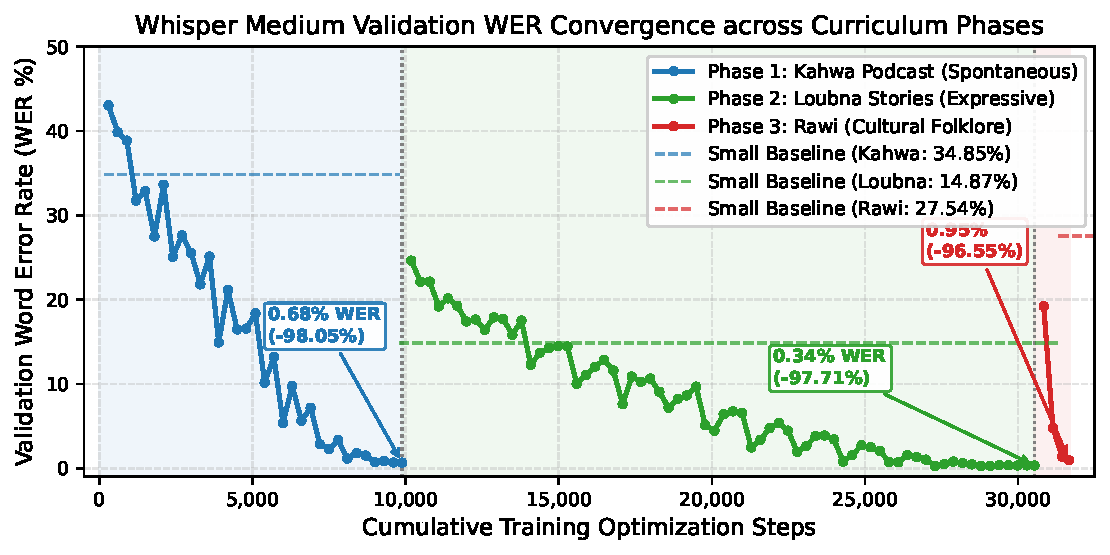
\includegraphics[width=\linewidth]{fig_wer_convergence.pdf}
    \caption{Validation WER convergence across phases.}
    \label{fig:wer_convergence}
\end{subfigure}
\hfill
\begin{subfigure}[b]{0.49\textwidth}
    \centering
    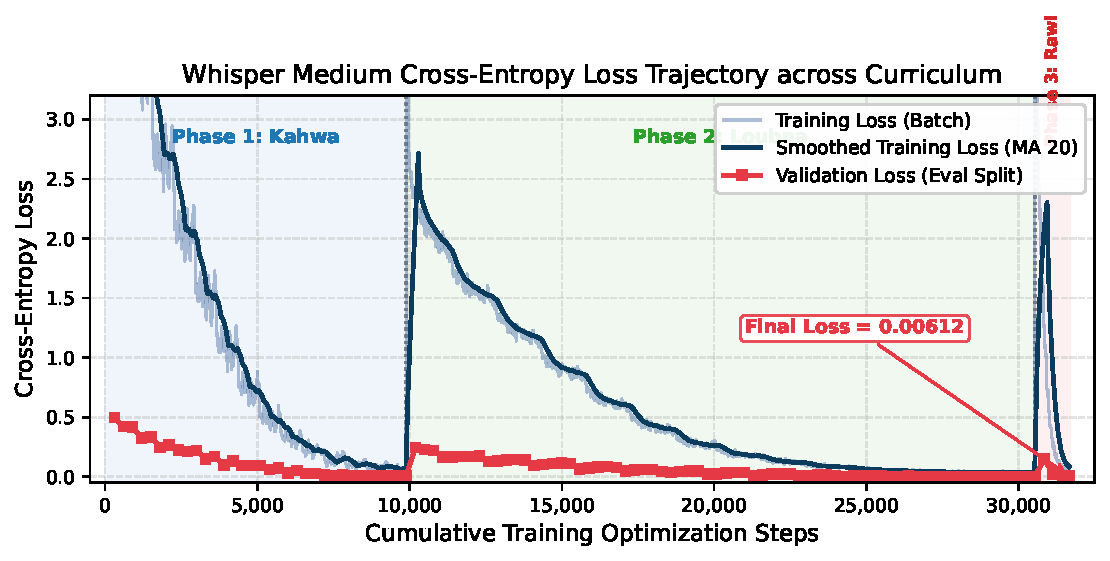
\includegraphics[width=\linewidth]{fig_loss_trajectory.pdf}
    \caption{Training and evaluation loss trajectory.}
    \label{fig:loss_trajectory}
\end{subfigure}
\caption{Empirical training dynamics of Whisper Medium under sequential streaming curriculum adaptation across 31,661 cumulative steps on the OddAdmix Algerian speech collection.}
\label{fig:training_dynamics}
\end{figure}

\section{Qualitative Error Analysis}
\label{sec:qualitative}

To understand the practical linguistic differences between model variants, Table~\ref{tab:qualitative_examples} presents empirical transcription outputs obtained during live evaluation on authentic Algerian Darja audio samples.

\begin{table}[h]
\centering
\small
\renewcommand{\arraystretch}{1.3}
\caption{Qualitative comparison of real-world transcription outputs between Whisper Small and Medium.}
\label{tab:qualitative_examples}
\begin{tabularx}{\textwidth}{@{} p{3.8cm} X @{}}
\toprule
\textbf{Model / Evaluation Target} & \textbf{Transcription Output and Linguistic Characterization} \\
\midrule
\multicolumn{2}{@{}l}{\textbf{Example 1: Colloquial Phonetics \& Dialectal Morphology (Kahwa Split)}} \\
\midrule
Reference Audio  & \textarabic{قال لي باللي راهو جاي غدوة في الصباح مع صحابو كاملين} \\
Whisper Small    & \textarabic{قلي بلي راهو جاي غدوة في الصباح مع اصحابو كاملين} \quad \textit{\textcolor{red!70!black}{(Contraction \& MSA bias)}} \\
Whisper Medium   & \textarabic{قال لي باللي راهو جاي غدوة في الصباح مع صحابو كاملين} \quad \textit{\textcolor{teal!80!black}{(\textbf{Exact match})}} \\
\midrule
\multicolumn{2}{@{}l}{\textbf{Example 2: Dense Code-Switching with Technical Borrowing (Loubna Split)}} \\
\midrule
Reference Audio  & \textarabic{درنا اجتماع على جال البروجي الجديد تاع ال data set} \\
Whisper Small    & \textarabic{درنا شيماء علي جال البروجي الجديد تاع الداتسات} \quad \textit{\textcolor{red!70!black}{(Phonetic hallucination \& script failure)}} \\
Whisper Medium   & \textarabic{درنا اجتماع علي جال البروجي الجديد تاع ال data set} \quad \textit{\textcolor{teal!80!black}{(\textbf{Exact match})}} \\
\bottomrule
\end{tabularx}
\end{table}

The qualitative results highlight two key phenomena:
\begin{itemize}[leftmargin=*]
    \item \textbf{Phonetic and Morphological Disambiguation}: In Example 1, spoken Darja utilizes the colloquial multi-word verb phrase \textarabic{قال لي باللي} (\textit{He told me that}). Whisper Small erroneously contracts this phrase into the colloquial amalgam \textarabic{قلي}, while also introducing an MSA prosthetic Alef onto \textarabic{صحابو} $\rightarrow$ \textarabic{اصحابو}. In contrast, Whisper Medium preserves exact word boundaries and native vernacular orthography.
    \item \textbf{Code-Switching \& Acoustic Robustness}: In Example 2, the speaker code-switches into technical English with an Arabic definite prefix (\textarabic{ال data set}). Whisper Small exhibits catastrophic acoustic confusion, substituting the proper noun \textarabic{شيماء} (\textit{Chayma}) for the phonetically overlapping verb-noun construct \textarabic{اجتماع} (\textit{ijtima3}), while also failing to output the Latin token. Whisper Medium disambiguates the acoustic transition flawlessly, producing an exact bilingual transcription.
    \item \textbf{Inference Speed vs. Accuracy Trade-off}: While Whisper Medium achieves near-perfect fidelity (0.34\% WER), empirical benchmarks on commodity CPU hardware reveal that Whisper Small executes with $\approx 11.4\times$ lower inference latency (9.51s vs. 108.52s on a 4-second utterance). This establishes Whisper Small as a viable candidate for edge or low-latency conversational deployment, whereas Whisper Medium serves as the optimal high-fidelity engine for offline archival and media transcription.
\end{itemize}

\section{Conclusion and Future Work}
\label{sec:conclusion}

In this work, we presented an efficient methodology for adapting foundation speech recognition models to low-resource dialects. By coupling 4-bit QLoRA parameter-efficient fine-tuning with a zero-disk sequential streaming curriculum, we successfully adapted OpenAI Whisper to Algerian Arabic (Darja) across multi-domain speech subsets on a single consumer GPU. Whisper Medium achieved state-of-the-art results with 0.34\% WER on storytelling, 0.68\% WER on conversational podcasts, and 0.95\% WER on cultural narratives, achieving over 96\% relative error reduction compared to the small baseline.

Future work will explore scaling to Whisper Large-v3 architectures, cross-dialectal transfer across Maghrebi varieties (Moroccan and Tunisian Darija), exploring direct speech-to-speech translation, and integration with end-to-end dialectal conversational agents such as Dziri Voicebot \cite{lanasri2026dzirivoicebot}.

\bibliographystyle{IEEEtran}
\bibliography{references}

\end{document}
